\graphicspath{ {02-CoordinateSystems/Figures/} }

\section{Coordinate systems}

\subsection{Laboratory coordinate system}

The origin of the LhARA coordinate system, the ``laboratory coordinate
system'' or ``laboratory reference frame'', is at the position of the
laser focus at the position of the laser-target interaction.
The $z$ axis is horizontal and points along the nominal capture axis,
pointing in the downstream direction, i.e. away from the target.
The $y$ axis is vertical, pointing vertically upwards, and the $x$
axis completes a right-handed coordinate system.

In the following, phase-space coordinates and vector and scalar
quantities referred to the laboratory coordinate system will be
written without a suffix.
Unit vectors along the $x$, $y$ and $z$ axes are $\bm{i}$, $\bm{j}$
and $\bm{k}$ respectively.

\subsection{Reference particle local coordinate system}

\begin{figure}
  \begin{center}
    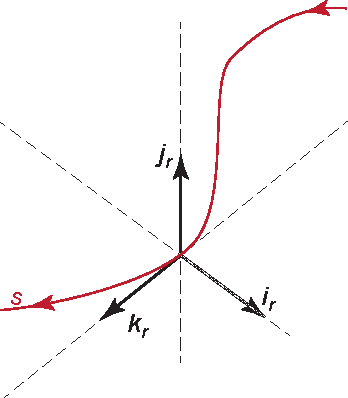
\includegraphics[width=0.55\linewidth]{RPLC.pdf}
  \end{center}
  \caption{
    Reference particle local coordinate system
  }
\end{figure}
